
\chapter{Literature review}

\section{Hydrogen impurity enrichment}
'Hydrogen impurity enrichment' is a term for any technique which involves increasing the 
concentration of impurities within a hydrogen sample by means of removing the hydrogen matrix gas. 
There are two previous reports of impurity enrichment being used as a technique for hydrogen impurity 
analysis. 
The first report by Papadis et al at Argonne National Laboratory used a Pd/Cu \cite{Ahmed2010}
coated Pd/Ag membrane for non-sulphur containing hydrogen samples and a Pd/Au coated Pd/Ag membrane for sulphur 
containing hydrogen samples to enrich impurities in a 50 bar sample. 
The analyte gas used contained 
N\textsubscript{2}, CH\textsubscript{4} and CO\textsubscript{2} at 100 \textmu mol/mol and an additional 
 2 \textmu mol/mol of H\textsubscript{2}S during sulphur tests sulphur. 
The enrichment was calculated by using measured values of temperature and pressure along with the 
non-ideal gas law, this was represented through a 'calculated enrichment factor' as shown in equations \ref{eq:1}
and \ref{eq:2}. 

\begin{equation} \label{eq:1}
    % \frac{(\frac{P_{1,a} V_1)}{Z_{1,a} RT_{1,a}})}
    CEF_{NI} = \frac{\frac{P_{1,a} V_1}{Z_{1,a}RT_{1,a}}\frac{P_{2,a} V_2}{Z_{2,a}RT_{2,a}}-\frac{P_{1,b} V_1}{Z_{1,b}RT_{1,b}}}{\frac{P_{2,b} V_2}{Z_{2,b}RT_{2,b}}}
\end{equation}

\begin{equation}\label{eq:2}
    y_{i,a} = \frac{y_{i,b}}{CEF}
\end{equation}
The set-up was able to reach enrichment factors of around 32 for non-sulphur tests and 15 
for sulphur tests. The non-sulphur tests closely matched with the actual component concentrations, 
however in the second set of tests there was some loss of sulphur observed, most likely due to the 
formation of palladium sulphide on the surface of the membrane, or through wall catalysed reactions. 

A similar experiment was performed by National Physical Laboratory with the aim of decreasing the uncertainty 
of using such a device. \cite{Murugan2014} The non-ideal gas law method used in the previous paper \cite{Ahmed2010} 
was compared to a novel tracer enrichment method developed by NPL. \cite{Murugan2014} 
The tracer enrichment method involves spiking the hydrogen sample with a known quantity of krypton prior to 
enrichment. The enrichment factor is then calculated using the change in concentration of the krypton as 
shown in equation \ref{eq:3}.

\begin{equation} \label{eq:3}
    CEF_{Tracer} = \frac{y_{kr_b}}{y_{Kr_b}} = \frac{1}{y_{Kr_a}} \frac{A_{Kr_b}}{A_{Kr_a}} y_{Kr_{st}}
\end{equation}

The set-up was similar to the one used by Papadias et al \cite{Ahmed2010} and was used to enrich a 50 bar 10L hydrogen sample 
containing 1.5-2 \textmu mol/mol of CO, Kr, CH\textsubscript{4} and N\textsubscript{2}. Use of the tracer enrichment 
method reduced the associated uncertainty from 2.6\% to 1\%. 
Two tests were performed, with the second test resulting in membrane failure. 

When operating the hydrogen impurity enrichment device it was found that both methods should be used to 
calculate the CEF.\cite{Murugan2014}\cite{Murugan2015} While the tracer enrichment method has a lower uncertainty 
due to it being dependant on fewer variables, it is impossible to tell if a leak has occurred in the device 
due to the covariance 
phenomena. \cite{Murugan2014} Leaks in the enrichment device could occur due to thermal expansion of components due to heating 
to the required operating temperature or cracks forming in the membrane. The stability of membranes used in 
such a device will be discussed in the following section. During a leak it will be expected that the ratio of 
krypton, along with other impurities which are not naturally present in air, will remain constant, resulting 
in no change in the CEF. A leak will allow oxygen and nitrogen to enter the system and throw off the 
measurement of these two impurities. While the tracer enrichment method could still be used to calculate 
the amount fraction of other impurities, the non-ideal gas law method would have to be used to provide an 
accurate measurement for Oxygen and Nitrogen.

A device similar to the HIED is the Hydrogen Elimination Mass Spectrometer (HEMS) designed by Power + Energy USA. \cite{Bossard} 
The principle behind the HEMS is the same as the HIED, where a palladium membrane is used to selectively 
remove the hydrogen matrix gas and thus concentrate the impurities within the hydrogen sample. 
The output is directly fed into a mass spectrometer which allows in-situ measurements to be performed. 
The limit of detection specified by the manufacturer claims to be in the range of pmol/mol however there is 
no published information regarding the accuracy or uncertainty associated with the device. 
As of 2016 the device was discontinued by the manufacturer.

\subsection{Criteria for a hydrogen impurity enrichment material}
In order for a membrane to be suitable for hydrogen impurity enrichment material it must be able to 
increase the concentration of low-level impurities in a hydrogen sample. 
Although all past examples of hydrogen impurity enrichment have used dense membranes with an infinite 
selectivity towards hydrogen, it is theoretically possible to use a membrane which has a lower selectivity 
to perform enrichment. This would have the advantage of allowing membranes with faster flux to be used, 
greatly reducing the amount of time required for an enrichment run, while allowing cheaper materials to be 
used in place of the palladium membranes used in past studies. In order to perform this calculation, 
the following must be known:
\begin{itemize}
\item Selectivity of the membrane must be known to a high accuracy
\item Total number of moles leaving the system
\item Concentration of enriched impurities
\end{itemize}

Since the selectivity shows the ratio of substances passing through the membrane 
(i.e. H\textsubscript{2}/N\textsubscript{2} selectivity of 2 represents 2 moles of hydrogen for every 1 mole 
of nitrogen passing through 
the membrane) if both quantities are known the number of moles of impurity leaving the system through 
permeation could be easily estimated.

\begin{equation}
    n_{i_{exit}} = n_{exit_{total}}/ \alpha^{H_2 /i}    
\end{equation}

The concentration, and therefore the number of moles of impurity on the retentate side of the membrane 
could then be analysed using suitable instrumentation. These values could then be added together and 
divided by the enrichment factor in order to give the original number of moles that would be in the vessel.

\begin{equation}
    y_i=\frac{(n_{i_{ret}}+n_{i_{exit}})/n_{tot_{ret}}}{CEF} 
\end{equation}

In practice however this may not be feasible due to the low concentrations of impurities expected to be 
present in these hydrogen samples. In order for an enrichment calculation to work there must be an analysable 
concentration of impurity remaining in order to back calculate. Since the level of expected impurities in a 
hydrogen sample is so low, and the selectivity of many membranes also low, there is a high risk of either all 
impurities simply leaving the sample during the enrichment run, or only achieving a lower enrichment factor. 
Take the example of enriching a sample containing 0.2 \textmu mol/mol of CO by 100 in order to analyse its 
composition on 
a GC-MS. If the sample is a standard 10L cylinder containing 100 bar a H\textsubscript{2}/CO selectivity of 
\textasciitilde 4950000 is required to simply prevent all of the CO leaving the enrichment device, which is 
effectively the 
same as the selectivity’s seen in dense metal membranes. However, for the same sample containing 0.3 \textmu mol/mol 
of 
Helium a H\textsubscript{2}/He selectivity of 330 is the minimum required which is more feasible. However, both these values 
are the exact values required by the standard, in reality they would be much lower. The highest reported 
selectivity of a non-infinitely selective membrane was Liquid crystalline polyester which had a 
H\textsubscript{2}/N\textsubscript{2} 
selectivity of  2632 \cite{Weinkauf1992} which indicates that this method may be suitable for enriching some of the higher 
concentration impurities in hydrogen samples, it is not a solution for lower concentration. 
It is also unlikely that the selectivity of a membrane material will stay constant throughout its lifespan. 
Any drift in selectivity would throw off the calculation and either require regular changing of the membrane, 
driving up cost, or regular calibration to recalculate the selectivity of the membrane at a given time, which 
would be time consuming. It is however likely that infinitely selective membranes are the only feasible 
enrichment material due to their ability to enrich every impurity in hydrogen, whereas non-infinitely 
selective membranes may be applied to analysis of individual impurities, it is unlikely such a scenario 
would occur in reality which makes them a non-ideal solution. 

\subsection{Other enrichment methods}
\subsubsection{Sorbent tubes}
The use of traps and sorbent tubes to pre-concentrate impurities in gases is very common in gas analysis, 
but only two hydrogen purity analysis standards have incorporated this technique to facilitate purity analysis. 
A method for concentrating the impurities in a sample of hydrogen using a zeolite- packed chromatographic 
column has been described in a paper by Hille \cite{Hille1990a}. The method involves flowing the gas sample into the column 
using a pump and cooling the column to a temperature that allows the impurities to remain trapped whilst the 
matrix gas passes through. The sample is then transferred to GC-MS for analysis. The enrichment factor for 
this method is determined by the flowrate and amount of time that the gas is sampled into the column. 
The method was validated by analysing gas mixtures of hydrogen containing 8.7 mmol/mol of silane. 
By enriching the sample, the signal- to-noise for the same measurement was increased by a factor of 2000 
indicating that levels in the range of 4 nmol/mol of silane would easily be measured using this method 
whereas the usual limit of detection (without pre-concentration) would have been 1 \textmu mol/mol

\subsubsection{Cryo-focusing}
A method for performing pre-concentration by cryo-focusing has been detailed in ASTM WK34574 
where the device is used to concentrate the impurities in a sample of hydrogen before introducing 
the gas to a GC-MS \cite{Murugan2015} The pre-concentration method involves trapping the impurities onto a glass bead trap 
at -150\textdegree C. By increasing the temperature of the trap all of the impurities apart from water 
are transferred to a separate Tenax trap which is cooled to -170\textdegree C. 
Upon heating once again the enriched sample is introduced to the analyser. 
Very high enrichment factors can be achieved using this method by flowing a high volume of the sample 
gas through the pre-concentration device to allow capture of the impurities whilst the hydrogen is removed. 
No information was provided in the standard to indicate the accuracy or limitations of this method.

\section{Review of hydrogen selective membranes}
The term membrane is used to describe a semipermeable barrier which selectively allows certain species to 
pass through it, while preventing or inhibiting the passage of others. The driving force for gas separation 
through a membrane is the pressure and component concentration gradients across the chosen material. 
In the context of hydrogen separation, the trans-membrane pressure and hydrogen concentration gradient 
across the feed and permeate, combined with the unique properties of the chosen separation material, 
will allow hydrogen to pass through the membrane, while preventing or inhibiting the transport of impurities 
which the membrane is not selective or less selective towards. A large number of materials have been studied 
for hydrogen separation. For the purpose of this review they will be split into four broad categories based 
on their material type and separation mechanism which is related to their pore structure (dense or porous); 
these categories are shown in Table 2 and visualized in Figure \ref{fig:1}.

The material, its structure with regards to pore size and pore size distribution, and surface chemistry, 
all contribute to the separation mechanism for removing hydrogen from its constituent gas mixture. 
The six main membrane separation mechanisms are visualised in Figure \ref{fig:1}, with (i) – (iv) showing the 
four separation mechanisms for gases in porous media, and (V)- (Vi) showing gas separation through dense media. 
For porous materials typically a combination of these mechanisms dictates the overall separation performance 
due to imperfections in the membranes structure. All dense membranes should be dictated by the solution 
diffusion mechanism and the presence of any other mechanisms are evidence of imperfections in the membrane. 

For most porous media, the separation mechanism is dominated by Poiseuille flow or Knudsen Diffusion. 
The precise separation mechanism can be determined by calculating the ratio between the mean free path of 
the gas molecules (\textlambda) and the pore radius (r) as shown in Equation \ref{eq:6} where \texteta \ is the viscosity of the gas, 
P is the pressure, T is the temperature, M\textsubscript{w} is the molecular weight of the gas, and R is the universal gas 
constant.

\begin{figure}
    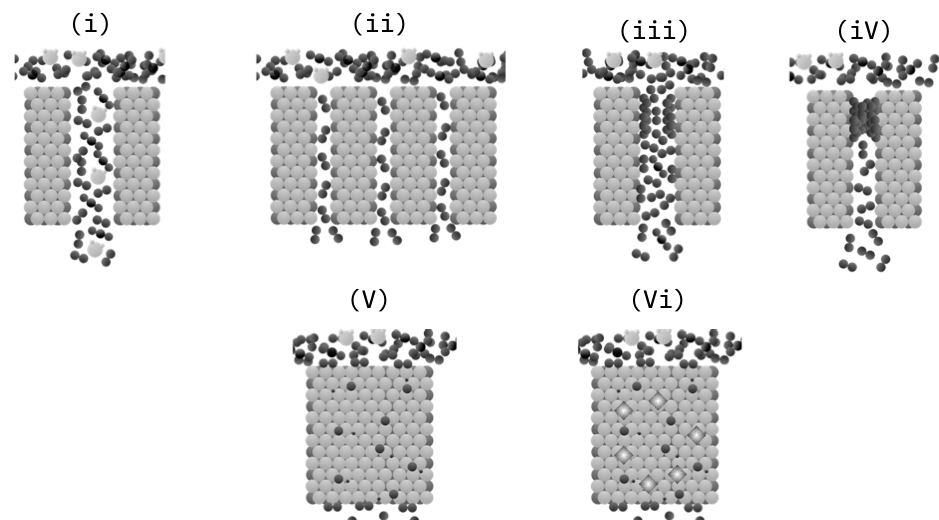
\includegraphics[width=\linewidth]{figures/septype.png}
    \caption{Illustration of the five membrane separation mechanisms (i) Poiseuille Flow/Knudsen diffusion, (ii) Molecular Sieving, (iii) Surface diffusion (iV) Capillary condensation (V) Solution diffusion (Vi) Facilitated transport}
    \label{fig:1}
  \end{figure}

\begin{equation}\label{eq:6}
    \frac{r}{\lambda} = \frac{2P}{3\eta}\sqrt{\left(\frac{2M_w}{\pi RT} \right)}
\end{equation}

This ratio determines the contribution of Knudsen and Poiseuille flow. If r/\textlambda \ > 1 it would indicate 
that the main gas transport rate limiting step is due to molecule-molecule collisions indicating that 
Poiseuille flow is the dominant transport mechanism. Likewise if r/\textlambda \ < 1 it indicates that 
molecule-wall collisions govern the rate limiting step showing that Knudsen diffusion is the dominant 
mechanism. If the transport is purely Knudsen diffusion the H\textsubscript{2}/CO\textsubscript{2} selectivity of 
the membrane will be equal to around 4.7. Since this value is relatively low, it has pushed researchers 
into fabricating membranes with smaller pore structures, and to modify their membranes to take advantage of 
specific surface interactions. Both of these developments allow researchers to surpass the selectivity 
achievable with purely Knudsen diffusion.

Molecular sieve materials can be classed as macroporous (>50nm), mesoporous (2-50nm) and microporous (<2nm) 
with microporous materials being the most relevant for hydrogen separation processes. These membranes are 
fabricated in such a way that the passageways are small enough that the entrance of molecules with large 
kinetic diameters is not possible. This results in higher permeation of smaller components in a gas mixture 
such as H2 or He while slowing, or completely preventing the passage of bulkier molecules. This mechanism, 
while effective for some gas mixtures, may not be feasible when looking to perform separation on similar 
sized gas pairs; selectivity is often hindered by competitive adsorption between the species due to the 
surface chemistry of the material. Fabrication of these membranes can also be difficult and manufacturing 
large scale membranes with a tight enough pore size distribution to ensure molecular sieving still proves 
to be a difficult task. Common microporous materials which are able to be fabricated into molecular sieving 
membranes are zeolites, metal organic frameworks, activated carbon, and amorphous silica.

Surface diffusion and capillary condensation are similar in that the surface chemistry of the pores in the 
membrane has a large effect on the separation efficiency. Surface diffusion occurs when the walls of the pore 
either intrinsically, or following modification, provides adsorption sites for the desired gas molecule. 
The gas molecule will adsorb onto the walls resulting in faster diffusion through the pore structure than 
other gases in the mixture. Similarly, capillary condensation typically follows on from surface diffusion 
and involves the gas species condensing within the pore of the membrane, either due to stronger molecule-wall 
interactions, or a smaller pore radius. The condensation of the molecule results in further selectivity 
improvements towards this component by providing an added transport barrier to other gas species. 

Gas transport in dense media is typically harder to categorise due to the unique material chemistry present 
in each material, however all dense membranes perform separation through some variation of the solution 
diffusion model. Typically, the following steps are always present in some form:
\begin{enumerate}
\item Adsorption of gas species onto the surface of the membrane 
\item Diffusion of gas species through the bulk of the membrane 
\item Desorption and diffusion of the gas species in the downstream. 
\end{enumerate}

More details will be provided on the precise features of solution diffusion in each material in the following 
sections. Facilitated transport is a sub section of solution diffusion and occurs in dense membranes which 
have a selected chemical species added into the bulk of the membrane. These materials are chosen based on the 
presence of a particular interaction with components of a gas species. These interactions are typically 
reversible reactions between the added species and the gas intended for separation and is intended to enhance 
the diffusion of the selected gas, this additive could either be fixed species (solid) or mobile (liquid). 

The most commonly reported metrics for membrane performance is the flux or permeability coefficient and 
selectivity. The flux (J) of a membrane is a measure of the amount of gas the membrane is allowing to pass 
per unit time per unit surface area and is typically used as a measure for how effective the fabricated 
membrane performs. The permeability coefficient (P) can be derived from the flux and is a quantitative 
expression which gives a specific measure of the separation properties of a material independent of 
operational and manufacturing constraints such as operating pressure and membrane thickness. 
While flux and permeability are similar and tied to each other they are both useful in their own way. 
The permeability coefficient is typically tied to the material and is useful for comparing different 
materials to each other, while the flux offers a measure on how effective the material is when fabricated 
into a membrane. 

The selectivity (\textalpha \ i/j) represents the separating ability of the membrane for a specific gas species 
(i) with respect to another gas species (j). This is common notation for porous membranes and membranes which 
are not completely selective towards one component. For membranes which are only selective towards one 
component such as dense metal and dense ceramic, the selectivity is not reported since any presence of 
another component in the exit stream is generally an indication of a manufacturing defect. 

While these values are reported for all membranes in order to allow for a direct comparison of 
performance, this is where the similarities end. The fundamental separation mechanism, manufacturing 
techniques, and unique material chemistry are often different for each material. In addition to this 
there are other important metrics for the usefulness of a membrane such as mechanical stability, lifespan, 
and chemical resistance which are more difficult to quantify. 


\subsection{Types of hydrogen separation membrane}
\begin{table}[htbp]
	\centering
	\caption{Types of hydrogen separation membrane}
	\resizebox{\textwidth}{!}{\begin{tabular}{LLLLLL}
		\hline
		\textbf{Material} & \textbf{Separation mechanism} & \textbf{Mechanical stability} & \textbf{Chemical Stability} & \textbf{Operating temperature} & \textbf{Selectivity} \\ \hline
		Polymer (Dense) & Solution diffusion, Facilitated transport &  Susceptible to Compaction 6 and Swelling 7
        & A & A & A \\
		Polymer (Porous) & Knudsen diffusion, Molecular sieving, Surface diffusion, Capillary condensation, Poiseuille flow  & Susceptible to Compaction 6 and Swelling 7 & Low chemical stability, Degrades under H\textsubscript{2}S, HCl, CO\textsubscript{2}, SO\textsubscript{x} 8
         & <100\textsuperscript{O}C & 2.5 9 –960 10
         (H2/N2 selectivity)         \\
		Nano-porous & Knudsen diffusion, Poiseuille flow, Capillary condensation, Surface diffusion, Molecular sieving & Brittle & Good 11 & Ambient -500\textdegree C & 2.4 12 -  1000 13
        (H2/N2 selectivity)
         \\
        Dense Metal & Solution Diffusion & Phase transition 14
        Dependant on support 14
        Surface segregation14
        & Negative interaction with CO, CH\textsubscript{4}, and H\textsubscript{2}O. Reacts with H\textsubscript{2}S and SO\textsubscript{x} 14 & 300-600 15 &  $\infty$ \\ 
        Dense Ceramic & Solution Diffusion & Brittle
        Difficult to seal due to high operating temperature
         & Degrades under CO\textsubscript{2} 16 & 500-1000 16
         & $\infty$ \\ \hline
	\end{tabular}}
\end{table}

\subsubsection{Micro-Porous materials}
Micro-porous materials are a class of materials generally used to refer to inorganic 
materials which possess small pores on a micrometre scale. Due to wide ranging scale of the 
term and the large volume of literature available on the following topics this section will 
aim to give a brief overview of each technology and identification of new trends in the field.
For more information on each topic the following reviews can be referred to for zeolites 
11,17–22, micro porous silica 11,17,23, carbon molecular sieve membranes 11,17,24–27, and 
Metal Organic Frameworks (MOFs).28–35 A direct comparison of recently reported micro-porous 
material membranes can be found in \textbf{'APPENDIX TABLE'}.

\paragraph{Zeolites} are a class of crystalline inorganic framework based on aluminosilicate minerals, 
and are the most widely resmearched class of micro-porous material. Zeolites are a popular 
choice for separation material due to their good thermal and chemical stability, and have 
been successfully applied to a number of fields including being fabricated into membranes 
for a range of gas separation applications.11 Zeolites can either occur naturally, or 
synthesised both at laboratory or industrial scale. 36  There are around 45 naturally 
occurring zeolites and an additional 232 synthetic zeolites, each given a three letter 
designation when approved by the International Zeolite Association Structure Commission. 37

The porosity and pore structure of a zeolite membrane is tightly tied to the chosen zeolite38. 
The final separation efficiency of a zeolite membrane is typically dictated by the method 
used to prepare it. In practice a zeolite membrane will have some degree of polycrystallinity 22,39 
due to the nature of the crystallisation based synthesis methods used. 
This will cause the formation of grain boundaries on the membrane, interrupting the 
homogeneity, and therefore the pore structure of the zeolite layer. One of the main 
challenges in scaling up production of zeolite membranes revolves around minimising or 
predicting the effects of this phenomena. 

Depending on the zeolite chosen, molecular sieving is possible assuming a continuous layer is 
deposited. In particular LTA 40 and MFI 41 show the greatest potential for hydrogen separation, 
showing separation performance surpassing that of Knudsen diffusion 42,43 and the ability to 
operate at temperatures ranging from ambient 42 to 500 \textdegree C 43. Current research 
trends still show that synthesis is the biggest target for researchers. 39 Some researchers 
have looked to 
the support as a place to improve the synthesis of zeolite membranes by incorporating 
3-aminopropyltriethoxysilan, PDA or ZnO into the inorganic support in order to improve 
adhesion, reduce the coarseness of the support, and enable the fabrication of thinner, 
more homogenous layers. The addition of these materials onto the support can also allow the 
support directing agent, and in some cases the seeding step altogether, too be bypassed. 
Minimising the use of support directing agent in the manufacture is advantageous since 
support directing agents typically slow the growth of zeolite, drive up cost and must be 
removed after synthesis, which could damage the membrane. 36 The addition of these materials 
on the support allows for covalent linkers to form between the support and zeolite, which 
assists the migration of zeolite particles during hydrothermal synthesis. 44

While zeolites have been researched for a number of decades and there have been many 
developments in microstructure tailoring, fabrication procedures, and thin film deposition, 
adoption of zeolite membranes have still been limited. This can mainly be attributed to the 
fact that the highest performing, and therefore most attractive, zeolite types are still 
difficult to synthesise on a large scale. While there has been some progress with the 
synthesis of sub-micron layers suitable for other separations, there is little published 
evidence that these layers are usable for the light gas separation required for large scale 
hydrogen production. Until this hurdle can be overcome it is unlikely that the technology 
can be used commercially. 45 Currently zeolite membranes have only been used commercially 
for liquid separation and with current research trends turning away from zeolites to newer 
classes of materials, their application may be limited to this area. This loss of interest 
is likely due to the lack of reproducibility to meet the standards required for industrial 
applications, therefore driving down the interest. 

\paragraph{Micro porous silica} membranes are amorphous structures which generally display tight pore 
size distributions and can be more easily fabricated into thin films than zeolites. They 
are an attractive option for large scale gas separations due to the low cost of the precursor 
materials required to fabricate the membrane. Silica membranes are typically composed of a 
three-layer structure; the membrane layer which is generally an ultra-microporous layer of 
the silica, an intermediary porous layer typically of the same silica material, and an 
inorganic porous support typically ceramic. Silica membranes are formed from networks of 
micropores typically on the scale of 0.5nm in diameter, giving them the potential to achieve 
molecular sieving separation similar to, or surpassing that of zeolites. 

From the membranes mentioned in Table 4 it is clear that silica membranes are an attractive 
option due to their extremely efficient separation characteristics. Silica membranes are able 
to achieve massive selectivity towards hydrogen, with some membranes reporting a H\textsubscript{2}/CO\textsubscript{2} 
selectivity greater than 1,000 46 with permeabilities on the scale of 10\textsuperscript{-7} mol/(m\textsuperscript{2} s pa) 
47. Many of the reported membranes are on the scale of \textless 100nm 47–49 which, if scalable, 
would result in a massive cost reduction when compared to other membrane types which require 
thicker layers to achieve usable separation performance. 

Silica membranes have been successfully applied on a lab scale however they experience 
stability issues, which must be overcome before they can be applied to a specific application. 
Silica membranes are highly unstable at high temperature and are easily attacked by moisture 
which causes the condensation of silanol groups in the silica layer, destroying the structured 
pores in the material. 50 The most common strategy to try and overcome this is to induce 
hydrophobicity to the membrane by incorporating a metal or metal oxide into the matrix.  
The thought process behind this is that the oxygen will form preferential bonds with the 
metal instead of the silanol group therefore maintaining pore structure. While this method 
seems promising, and may improve performance, it is unclear from literature if any long term 
stability studies have been performed to test if this is a lasting improvement. The most 
common metal dopants for this purpose are cobalt 47,51, iron, nickel and niobium 46,52. 
Additionally hydrophobicity could be induced by replacing some of the silanol groups on the 
surface of the membrane with carbon groups as shown by Lee 13,48,53. 

\paragraph{Carbon based membranes} come in many forms with the most common being carbon 
molecular sieve membranes but can also be extended to graphene. 

In theory any carbon containing compound could be used to manufacture a carbon molecular 
sieve membrane, however synthetic polymers are typically preferred due to their ability to 
be easily processed into homogeneous films which are essential for forming a homogenous 
carbon film.26  The precursor material should also show good thermal stability and not melt 
or soften during the pyrolysis step, again to ensure a homogenous carbon layer is formed. 25

Carbon molecular sieve membranes are typically stable in most environments, however suffer 
in the presence of oxygen and water due to the materials readiness to oxidation. 27 Due to 
this carbon molecular sieve membranes typically see large permeability reduction when exposed 
to small levels of these impurities. 27

Although zeolites and MOF’s often show higher separation performance than carbon molecular 
sieves, their high fabrication cost limits their use to processes with high margins. 
Carbon molecular sieve membranes can overcome the limitations of other porous materials 
while theoretically maintaining a cost similar to that of polymer membrane systems. 24 
While the theoretical cost of producing carbon molecular sieve membranes is low, its current 
cost is high due to the popularity of polyimide as a precursor. Since many carbon molecular 
sieve membranes are manufactured from polymers which are already used in the fabrication of 
polymer membranes it is unlikely that choosing to make them into carbon molecular sieve 
membranes will be an economical option. In order for the technology to flourish in industry 
alternative precursors must be researched and commercialised. 

Graphene and its variations have also seen some success when applied to hydrogen separation. 
Graphene is the term used to refer to a single layer of sp2 hybridised carbon. Due to the 
ultrathin nature of graphene, along with its strong mechanical and chemical stability, it 
makes an extremely attractive choice for a membrane material. 54 A dense layer of graphene 
is completely impermeable to gases and therefore further modification is required in order 
to bring about any separation behaviour. 55 Gas separation behaviour in graphene membranes 
is normally induced through the introduction of defects, this can either be defects which 
are present from the manufacturing process as shown in the papers published by Kim 56 and Zhu 57, 
or through post treatment of a dense graphene layer commonly through methods such as 
ultraviolet induced oxidative etching or oxygen plasma etching as performed by Celebi et al. 
58 While these techniques have the potential for producing high performing membranes, 
synthesising pristine, large area, graphene on a large scale still remains a problem and 
even small areas are costly to produce. 55  The defect-based nature of graphene based 
membranes also makes their commercial use questionably as there is little evidence that 
many of the reported membranes have repeatable performance characteristics. It may be that 
many of the reports are statistical anomalies and the technology simply will not show the 
repeatability to provide a commercial solution for light gas separations.

\paragraph{Metal-organic frameworks} are a new class of porous material. Similar to zeolites 
the material displays an intrinsic porosity, however unlike zeolites MOF’s have the additional 
advantage that their structures are highly tuneable past the porosity achieved intrinsically 
through the crystalline structure. 28 MOFs are compounds which consist of a metal ion, or 
clusters of metal ions, coordinated to organic ligands to form one, two- or three-dimensional 
structures. The study of MOFs is similar to zeolites and due to the field’s infancy, takes 
much inspiration from the zeolite field. For this reason, the field was able to develop 
quickly on the back of already established methods. MOF’s are unique in that their structures 
are more flexible than that of zeolites which would allow their separation properties to 
change with the operating conditions including temperature, humidity and light. 

Due to the resurgence of the hydrogen economy in recent years there have been many reports of 
the application of MOF membranes for the selective permeation of hydrogen. Due to the tuneable 
nature of MOF’s, the field comprises of two main concepts when developing a new membranes, 
taking advantage of the size and shape selectivity of the chosen MOF to enhance molecular 
sieving behaviour, and optimising the preferential adsorption properties of the MOF to enable 
improved separation properties through capillary condensation and surface diffusion. 

In particular ‘zeolitic immobilized frameworks’ or ZIF’s have seen particular interest in the 
hydrogen separation field. ZIFs are a class of metal organic framework which topologically 
have the same crystalline structure as zeolites, while still allowing for the fine-tuned 
separation properties seen in other MOFs. ZIF’s are often applied to hydrogen separation 
applications due to its high stability and affinity towards adsorption of hydrogen. ZIF-8, 
which appears to be the most popular choice for fabrication of MOF membranes for hydrogen 
separations in recent years, has a pore size of around 3.4Å and has been successfully applied 
to hydrogen separations, however results vary a lot with reported permeability values for the 
MOF ranging from as high as  2.1x10 \textsuperscript{-5} mol/(m\textsuperscript{2} s pa) 59 
to as slow as 6.59x10\textsuperscript{-8} mol/(m\textsuperscript{2} s pa) 60 depending on the 
operating conditions. This variability is also seen in the selectivity with reported H2/CO2 
selectivity’s ranging from 4 60 to 25 61, showing, that similar to zeolites, the field still 
has some consistency issues with the fabrication step which must be resolved before scaling 
up. 
\renewcommand{\bibname}{References}

\bibliographystyle{unsrtnat}



\bibliography{library.bib}